\section{Problem Definition \label{ProblemDefinition} }
This section will further specify the challenges of the defined main contributions of this project. Each definition will be addressed further in \secref{Implementation}.\\

\textbf{Data Acquisition Controller:} This part of the project is about developing a controller that can collect sensor data from within a simulation environment. It is important to avoid gathering unnecessary data and to avoid collision, which guarantees a fluent and efficient process. Both requirements can be reached with specific algorithms, that record sensor inputs, while applying all required conditions. To properly complement images to current and futuer laser input, the robot moves towards an obstacle in a straight line. This is crucial, as if the recording is taking place on a straight trajectory, the obstacles itself, do not change. The obstacles are merely displayed as a larger entity, on the recorded images. This concept allows relating images to current and future laser data. If the recording would not be on a straight line, every recording would contain differnt obstacle entities. \figref{relate_data} depicts a robot in rear view, moving towards an obstacle in a straight line while recording images.\cite{nava2019learning} suggests this concept, which will be discussed further in \secref{DataAcquisition}.

\begin{figure}[h]%[htbp]
\centering
\captionsetup{width=.75\linewidth}
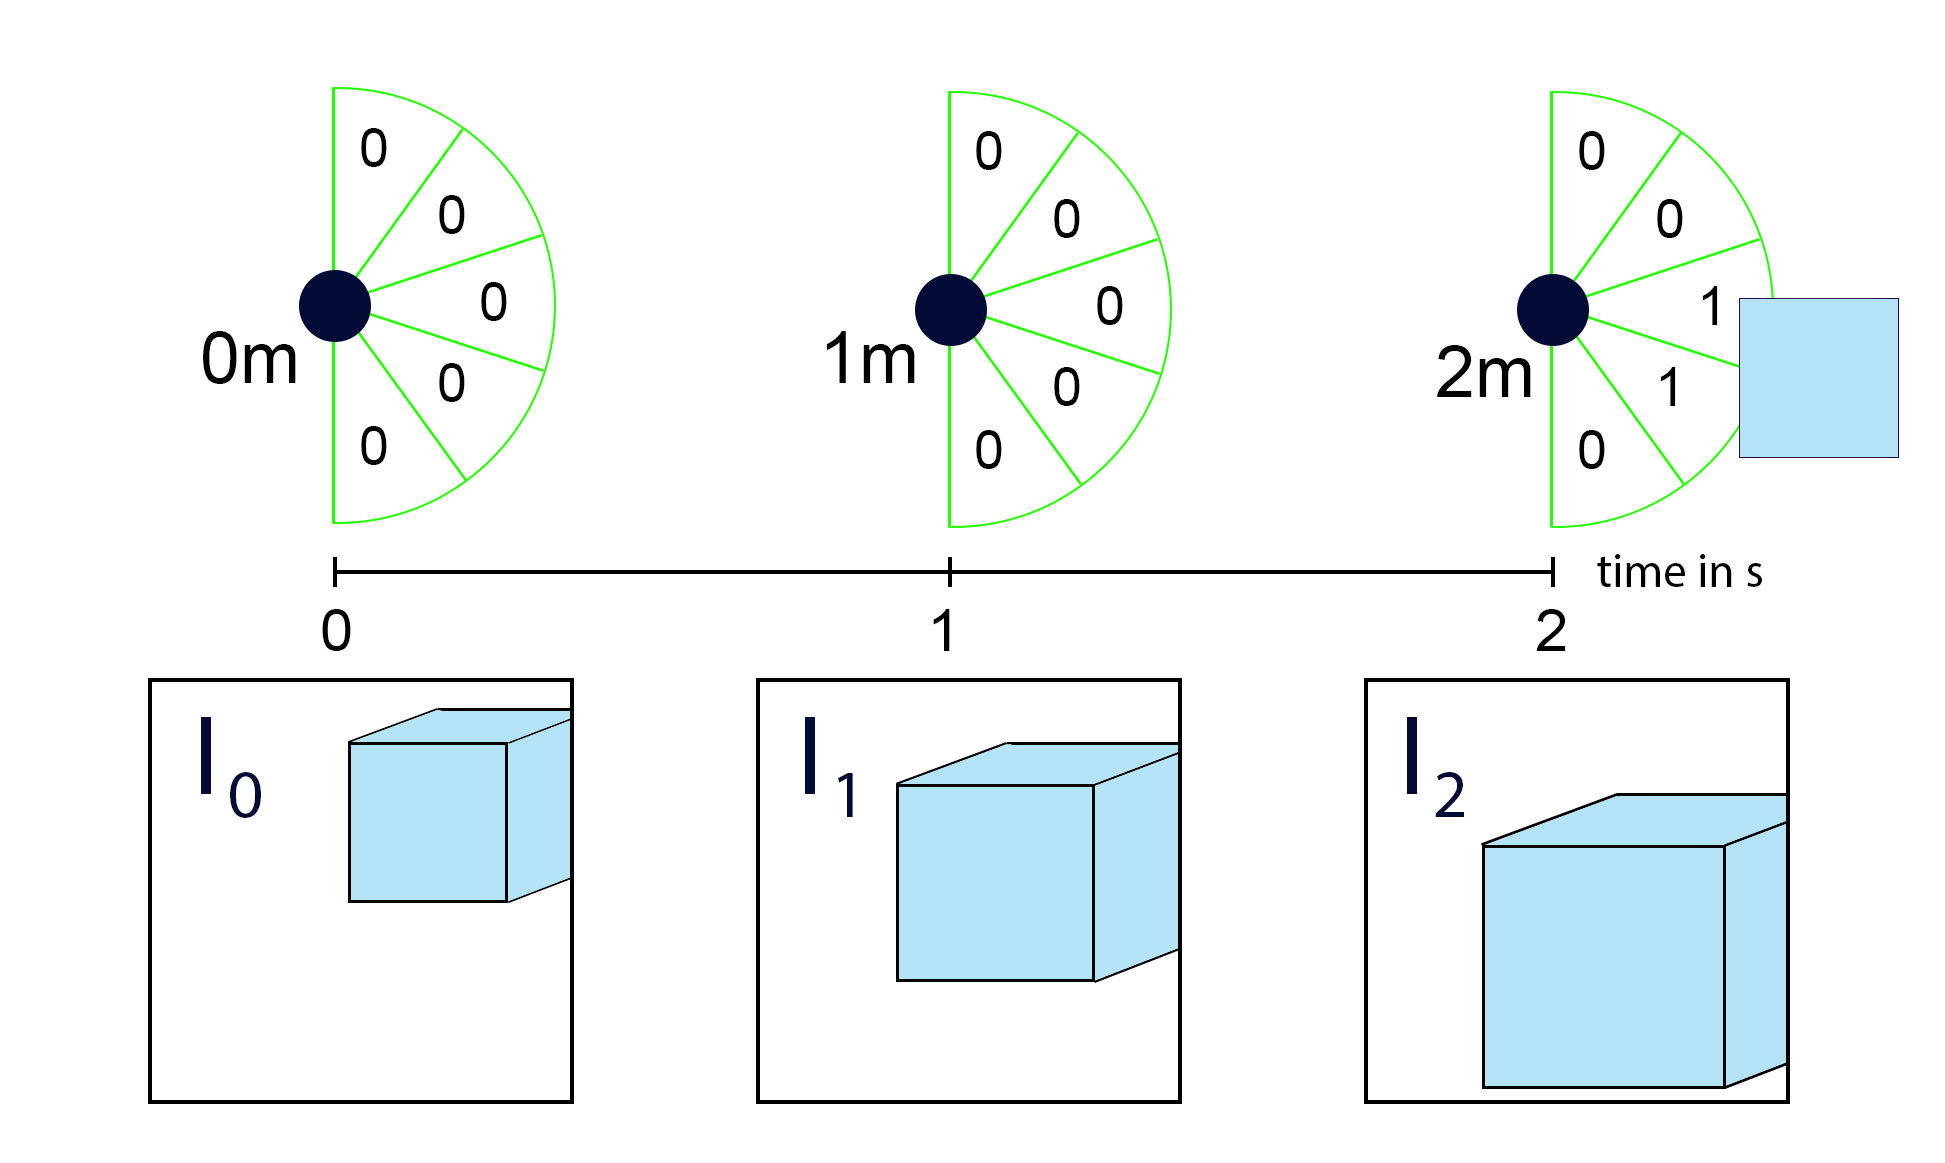
\includegraphics[width=0.75\linewidth]{Bilder/Relate_data.png} 
\caption{Concept of how images at time $t_{0}$ can be related to future laser input, if recording is taking place on a straight line. The obstacle entities are the same, but the image representations are getting larger.}
\label{relate_data}
\end{figure}

\textbf{Feature Extraction:} This step is about the autonomous creation of a dataset. The challenge is to relate images recorded at a specific time t to future laser input. The laser input is provided by a laser scanner, which returns information about recorded distances of obstacles in its vicinity. To simplify the laser input, laser distances are transferred to binary labels. To obtain binary labels for training, laser elements, need to be divided in up to n ranges, and distances to binary values if they are smaller than a specific threshold. To provide a more robust and reliable dataset, images recorded at time $t_{0}$ are not just related to laser input at time $t_{0}$, but also to laser information at future times. The concept of this can be seen at \figref{relate_data} and its corresponding table at \figref{dataset_table}, where each camera input is related to current and future laser input.

\begin{figure}[h]%[htbp]
\centering
\captionsetup{width=.75\linewidth}
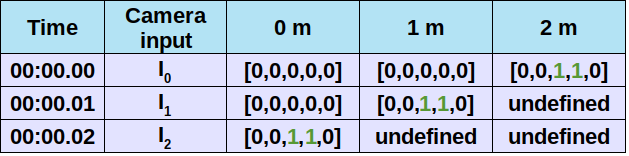
\includegraphics[width=0.75\linewidth]{Bilder/dataset_table.png} 
\caption{Finished dataset table relating images with future laser data.}
\label{dataset_table}
\end{figure}

\textbf{Training Environment:} This part is about the training of a Neural Network. As the dataset provides image data as input, the pipeline's training stage uses a Convolutional Neural Network. The entire pipeline but especially this part, is expected to be used iteratively to increase the performance of a trained model by adjusting the network's parameters.\\

\textbf{Testing:} The testing stage is about the implementation of performance metrics, to gain information about which parameters require modifications. This stage includes different types of scenarios, like the calculation of the Area under the Curve, the Analysis of a Simulated Prototype, or Visualized Models. These scenarios are highly critical to get an insight into the model's performance or hints of where to adapt, change, or replace parameters or functions.\\

\textbf{Performance Monitoring:}
At this stage of the pipeline, testing results from all previous stages are analyzed, interpreted, and documented. It further administrates all files created, continuously checks the pipeline for consistency, or tries to recognize bottlenecks or other errors, which cause the pipeline to slow down or fail. This stage is crucial, as based upon the insights given, the practitioner can decide where to change, add or adjust functions or parameters.\\

\textbf{Obstacle Avoidance Controller:} Once the model is trained, tested, and ready for deployment, it will be served as the core of an obstacle avoidance controller, which provides the model with new input data and expects it to predict reliable output about obstacles around the robot's vicinity. It is important to note that camera input alone will serve as input. At this final stage, no laser information is used.
